\documentclass[11pt,a4paper]{article}
\usepackage{gtu-el-yazisi}
\begin{document}
\notbilgi{Analog Haberleşme}{Uygulama 2: LTI kanal, AM ve çoklama}{Analog-Uygulama-2.pdf}

\sayfa{1}
\begin{ornek}
$x(t)=2\,\mathrm{sinc}(40t)$ işareti transfer fonksiyonu $H(f)$ olan bir kanaldan iletilmektedir.
$y(t)=20\,\mathrm{sinc}(40t-200)$ old. göre,
\begin{enumerate}[label=\alph*)]
\item $H(f)$'yi bulun. Genlik ve faz spektrumlarını çiziniz
\item $h(t)$'yi bulun
\item Bu sistem bozulmasızmıdır? \\ $x(t)=t\,\mathrm{sinc}^2(t)$ ise $y(t)=\,$?
\item $x(t)=2\,\mathrm{sinc}(40t)$ için, çıkışın enerji spektral yoğunluğunu bulun
\item Çıkış işaretinin enerjisini bulun.
\end{enumerate}
\end{ornek}

\begin{center}
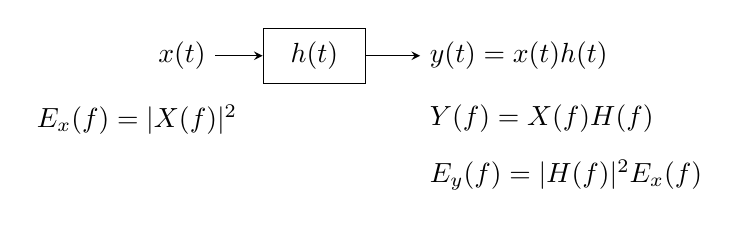
\begin{tikzpicture}[>=stealth]
\node[anchor=east] (x) at (0,0) {$x(t)$};
\node[draw,anchor=west,minimum width=1.3cm,minimum height=0.7cm] (h) at (0.6,0) {$h(t)$};
\node[anchor=west] (y) at (2.6,0) {$y(t)=x(t)\circledast h(t)$};
\draw[->] (x.east) -- (h.west);
\draw[->] (h.east) -- (y.west);
\node[anchor=north east] at (0.4,-0.5) {$E_x(f)=|X(f)|^2$};
\node[anchor=north west] at (2.6,-0.5) {$Y(f)=X(f)H(f)$};
\node[anchor=north west] at (2.6,-1.2) {$E_y(f)=|H(f)|^2E_x(f)$};
\end{tikzpicture}
\end{center}

\formulkutu{\begin{aligned} x(t-t_0) &\overset{\mathcal F}{\longleftrightarrow} X(f)\,e^{-j2\pi f t_0}\\ A\tau\,\mathrm{sinc}(\tau t) &\overset{\mathcal F}{\longleftrightarrow} A\,\Pi\!\left(\frac{f}{\tau}\right)\end{aligned}}

\[ \text{a)}\quad x(t)=2\,\mathrm{sinc}(40t)\ \underset{\substack{\tau=40\\ A\tau=2\\ A=1/20}}{\overset{\mathcal F}{\longleftrightarrow}}\ X(f)=\frac{1}{20}\,\Pi\!\left(\frac{f}{40}\right) \]

\begin{center}
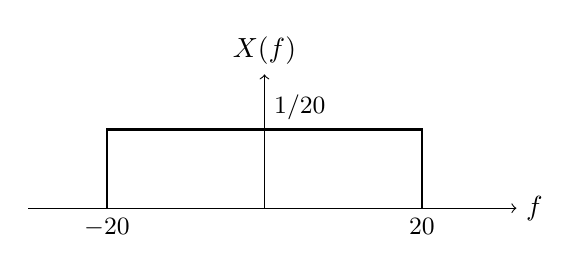
\begin{tikzpicture}[x=0.1cm,y=1cm]
\draw[->] (-30,0) -- (32,0) node[right] {$f$};
\draw[->] (0,0) -- (0,1.7) node[above] {$X(f)$};
\draw[thick] (-20,0) -- (-20,1) -- (20,1) -- (20,0);
\node[above right] at (0,1) {\small $1/20$};
\node[below] at (-20,0) {\small $-20$};
\node[below] at (20,0) {\small $20$};
\end{tikzpicture}
\end{center}

\[ y(t)=20\,\mathrm{sinc}\bigl(40(t-5)\bigr)\ \underset{\substack{\tau=40\\ A=1/2}}{\overset{\mathcal F}{\longleftrightarrow}}\ Y(f)=\frac{1}{2}\,\Pi\!\left(\frac{f}{40}\right)e^{-j2\pi f\,5} \]
\[ H(f)=\frac{Y(f)}{X(f)}=10\,\underbrace{\Pi\!\left(\frac{f}{40}\right)}_{\text{yine kare darbe gelir}}\,e^{-j2\pi f\,5} \]

\begin{center}
\begin{tikzpicture}[x=0.1cm,y=0.1cm]
\draw[->] (-30,0) -- (32,0) node[right] {$f$};
\draw[->] (0,0) -- (0,16) node[above] {$|H(f)|$};
\draw[thick] (-20,0) -- (-20,10) -- (20,10) -- (20,0);
\node[above left] at (0,10) {\small $10$};
\node[below] at (-20,0) {\small $-20$};
\node[below] at (20,0) {\small $20$};
\begin{scope}[xshift=9cm]
\draw[->] (-30,0) -- (32,0) node[right] {$f$};
\draw[->] (0,-16) -- (0,16) node[above] {$\Theta_H(f)$};
\draw[thick] (-24,19) -- (24,-19) node[below right] {\small $-10\pi f$};
\end{scope}
\end{tikzpicture}
\end{center}

\[ \text{b)}\quad h(t)=400\,\mathrm{sinc}\bigl(40(t-5)\bigr) \]

\noindent c) Bozulmasızdır. (Çünkü giriş işareti için) genlik spektrumu sabit, faz spektrumu lineerdir.

\begin{center}
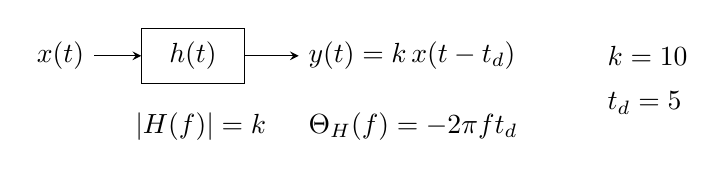
\begin{tikzpicture}[>=stealth]
\node[anchor=east] (x) at (0,0) {$x(t)$};
\node[draw,anchor=west,minimum width=1.3cm,minimum height=0.7cm] (h) at (0.6,0) {$h(t)$};
\node[anchor=west] (y) at (2.6,0) {$y(t)=k\,x(t-t_d)$};
\draw[->] (x.east) -- (h.west);
\draw[->] (h.east) -- (y.west);
\node[anchor=north west] at (0.4,-0.6) {$|H(f)|=k$};
\node[anchor=north west] at (2.6,-0.6) {$\Theta_H(f)=-2\pi f t_d$};
\node[anchor=west] at (6.4,0) {$k=10$};
\node[anchor=west] at (6.4,-0.6) {$t_d=5$};
\end{tikzpicture}
\end{center}

\sayfa{2}
\begin{gather*}
x(t)=t\,\mathrm{sinc}^2(t)\\
y(t)=10\,x(t-5)=10\,(t-5)\,\mathrm{sinc}^2(t-5)
\end{gather*}

\[ \text{d)}\quad x(t)=2\,\mathrm{sinc}(40t) \]
\begin{align*}
E_x(f)&=|X(f)|^2=\frac{1}{400}\,\Pi\!\left(\frac{f}{40}\right)\\
&=\frac{1}{4}\,\Pi\!\left(\frac{f}{40}\right)\footnotemark
\end{align*}
\footnotetext{Claude notu: ikinci satır muhtemelen $E_y(f)=|H(f)|^2E_x(f)=100\cdot\frac{1}{400}\,\Pi\!\left(\frac{f}{40}\right)$ olmalı.}

\begin{center}
\begin{tikzpicture}[x=0.1cm,y=1cm]
\draw[->] (-30,0) -- (32,0) node[right] {$f$};
\draw[->] (0,0) -- (0,1.7) node[above] {$E_y(f)$};
\draw[thick] (-20,0) -- (-20,1) -- (20,1) -- (20,0);
\node[above right] at (0,1) {\small $1/4$};
\node[below] at (-20,0) {\small $-20$};
\node[below] at (20,0) {\small $20$};
\end{tikzpicture}
\end{center}

\begin{align*}
\text{e)}\quad E_y&=\int_{-\infty}^{\infty}E_y(f)\,df\\
&=\int_{-20}^{20}\frac{1}{4}\,df=\frac{1}{4}\cdot 40=10\ \mathrm{J}
\end{align*}

\begin{ornek}
Bir LTI sistem olarak modellenen kanalın dürtü cevabı, $h(t)=5\,\delta(t-10)$ olarak verilmektedir.
\begin{enumerate}[label=\alph*)]
\item Bu sistemin Transfer fonksiyonunu bulun. Genlik ve faz spektrumlarını çizin. \\ Bu sistem bozulmasız mıdır? Neden??
\item $x(t)=10+10t\,\mathrm{sinc}(t)$ işareti uygulanırsa çıkışı nedir
\item $x(t)=20\cos(2000\pi t)+10\sin(4000\pi t)$ ise $x(t)$'nin güç yoğunluk fonksiyonunu (power spectral density) bulun
\item c şıkındaki $x(t)$ için $y(t)$'yi ve $y(t)$'nin GYF'sini bulun.
\item $y(t)$'nin özilişki fonksiyonunu bulun
\item $y(t)$'nin gücünü hem özilişki fonksiyonundan hem de GYF'den bulun.
\end{enumerate}
\end{ornek}

\[ \text{a)}\quad h(t)=5\,\delta(t-10)\ \overset{\mathcal F}{\longrightarrow}\ H(f)=5\,e^{-j2\pi 10f} \]
\begin{gather*}
H(f)=|H(f)|\,e^{j\Theta_H(f)}\\
|H(f)|=5 \qquad \Theta_H(f)=-2\pi\,10f
\end{gather*}

\begin{center}
\begin{tikzpicture}[x=0.1cm,y=0.15cm]
\draw[->] (-30,0) -- (32,0) node[right] {$f$};
\draw[->] (0,-4) -- (0,14) node[above] {$|H(f)|$};
\draw[thick] (-30,5) -- (30,5);
\node[above right] at (0,5) {\small $5$};
\begin{scope}[xshift=9cm]
\draw[->] (-30,0) -- (32,0) node[right] {$f$};
\draw[->] (0,-12) -- (0,14) node[above] {$\Theta_H(f)$};
\draw[thick] (-20,12) -- (20,-12) node[below right] {\small $-20\pi f$};
\end{scope}
\end{tikzpicture}
\end{center}

Genlik spektrumu sabit, faz spektrumu lineer olduğu için sistem bozulmasızdır.

\sayfa{3}
\begin{align*}
\text{b)}\quad x(t)&=10+10t\,\mathrm{sinc}(t)\\
y(t)&=k\,x(t-t_d)=5\,x(t-10)\\
&=50+50(t-10)\,\mathrm{sinc}(t-10)
\end{align*}

\begin{align*}
x(t)&=\sum_n x_n\,e^{j2\pi n f_0 t}\\
R_x(\tau)&=\sum_n |x_n|^2\,e^{j2\pi n f_0 \tau} & \cos(a)&=\tfrac12\left[e^{-ja}+e^{ja}\right]\\
\overset{\mathcal F}{\downarrow}\quad S_x(f)&=\sum_n |x_n|^2\,\delta(f-nf_0)
\end{align*}

\begin{align*}
\text{c)}\quad x(t)&=20\cos(2\pi\,1000\,t)+10\sin(2\pi\,2000\,t)\\
&=\underbrace{10\,e^{-j2\pi 1000t}}_{x_{-1}}+\underbrace{10\,e^{j2\pi 1000t}}_{x_{1}}+\underbrace{\frac{10}{2j}\,e^{j2\pi 2000t}}_{x_{2}}\\
&\quad\underbrace{-\frac{10}{2j}\,e^{-j2\pi 2000t}}_{x_{-2}}
\end{align*}
\[ S_x(f)=100\,\delta(f-1000)+100\,\delta(f+1000)+25\,\delta(f-2000)+25\,\delta(f+2000) \]

\begin{align*}
\text{d)}\quad y(t)&=5\,x(t-10)\\
&=100\cos\bigl(2\pi\,1000\,(t-10)\bigr)+50\sin\bigl(2\pi\,2000\,(t-10)\bigr)\\
S_y(f)&=|H(f)|^2S_x(f)=25\,S_x(f)=2500\bigl[\delta(f-1000)+\delta(f+1000)\bigr]\\
&\quad+625\bigl[\delta(f-2000)+\delta(f+2000)\bigr]
\end{align*}

\[ \text{e)}\quad R_y(\tau)=5000\cos(2\pi\,1000\,\tau)+1250\cos(2\pi\,2000\,\tau) \]

\[ \text{f)}\quad P_y=\int_{-\infty}^{\infty}S_y(f)\,df=R_y(0) \]
\formulkutu{R_y(\tau)=\int_{-\infty}^{\infty}S_y(f)\,e^{j2\pi f\tau}\,df}
\[ P_y=R_y(0)=6250 \]

\begin{ornek}
Fourier spektrumu $M(f)=\Pi(f/20)$ olan mesaj işareti aşağıda verilen sistemden geçmektedir. $x(t)$, $y_1(t)$, $y_2(t)$, $y_3(t)$ ve $y_4(t)$'ü zaman ve frekans domaininde ifade ediniz, spektrumlarını çiziniz.
\end{ornek}
\formulkutu{f_c\gg B}

\begin{center}
\begin{tikzpicture}[>=stealth,font=\small]
\node[anchor=east] (min) at (0,0) {$m(t)$};
\node[draw,circle,inner sep=1pt] (m1) at (1.2,0) {$\times$};
\node[draw,align=center,minimum width=1.6cm,minimum height=0.9cm] (b1) at (3.6,0) {kare\\ alıcı};
\node[draw,align=center,minimum width=1.7cm,minimum height=1.1cm] (b2) at (6.6,0) {BGF\\ B.G.\,$=4B$\\ $M=2f_c$};
\node[draw,circle,inner sep=1pt] (m2) at (9.0,0) {$\times$};
\node[draw,align=center,minimum width=1.4cm,minimum height=0.9cm] (b3) at (11.0,0) {AGF\\ B.G.\,=\okunamadi{2B}};
\node[anchor=west] (mout) at (12.0,0) {$y_4(t)$};
\draw[->] (min.east) -- (m1.west);
\draw[->] (m1.east) -- node[above] {$x(t)$} (b1.west);
\draw[->] (b1.east) -- node[above] {$y_1(t)$} (b2.west);
\draw[->] (b2.east) -- node[above] {$y_2(t)$} (m2.west);
\draw[->] (m2.east) -- node[above] {$y_3(t)$} (b3.west);
\draw[->] (b3.east) -- (mout.west);
\draw[->] (1.2,-1.0) -- (m1.south);
\node[below] at (1.2,-1.0) {$\cos(2\pi f_c t)$};
\draw[->] (9.0,-1.0) -- (m2.south);
\node[below] at (9.0,-1.0) {$4\cos(4\pi f_c t)$};
\draw[dashed,kirmizikalem] (7.75,1.3) -- (7.75,-2.0);
\node[turuncukalem,font=\scriptsize] at (2.6,1.4) {$x$'i $x^2$ yapıyor};
\draw[->,turuncukalem] (3.0,1.15) -- (3.3,0.5);
\draw[kirmizikalem] (0.2,-1.95) -- (0.2,-2.05) -- (7.5,-2.05) -- (7.5,-1.95);
\draw[kirmizikalem] (8.0,-1.95) -- (8.0,-2.05) -- (12.6,-2.05) -- (12.6,-1.95);
\node[kirmizikalem] at (3.9,-2.45) {Modülasyon};
\node[kirmizikalem] at (10.3,-2.45) {Demodülasyon};
\end{tikzpicture}
\end{center}

\sekilnotu[3]{Sayfanın altında turuncu kalemle spektrum taslakları başlamış ve sayfa sonunda kesilmiş: solda ``BGF'' başlıklı eksen üzerinde $2f_c-2B$, $2f_c$, $2f_c+2B$ noktalarıyla işaretli dikdörtgen biçimli bir bant; sağda $-2B$ ve $2B$ ile işaretli dikdörtgen biçimli bir spektrum taslağı. Turuncu oklar BGF ve AGF bloklarından bu taslaklara iniyor.}

\sayfa{4}
\[ M(f)=\Pi\!\left(\frac{f}{2B}\right) \]
\begin{center}
\begin{tikzpicture}[>=stealth,font=\small]
\draw[->] (-2.2,0) -- (2.4,0) node[right] {$f$};
\draw[->] (0,0) -- (0,1.5) node[above] {$|M(f)|$};
\draw[thick] (-1,0) -- (-1,0.8) -- (1,0.8) -- (1,0);
\node[below] at (-1,0) {$-B$};
\node[below] at (1,0) {$B$};
\end{tikzpicture}
\end{center}

\begin{align*}
M(f)&=\Pi\!\left(\frac{f}{2B}\right)\\
\hookrightarrow\ m(t)&=2B\,\mathrm{sinc}(2Bt)\\
&=2B\,\mathrm{sinc}(2Bt)\cos(2\pi f_ct)\footnotemark
\end{align*}
\footnotetext{Claude notu: ikinci satır muhtemelen $x(t)=m(t)\cos(2\pi f_ct)=2B\,\mathrm{sinc}(2Bt)\cos(2\pi f_ct)$ olmalı.}
\begin{gather*}
X(f)=\frac12 M(f-f_c)+\frac12 M(f+f_c)\\
X(f)=\frac12\,\Pi\!\left(\frac{f-f_c}{2B}\right)+\frac12\,\Pi\!\left(\frac{f+f_c}{2B}\right)
\end{gather*}

\begin{center}
\begin{tikzpicture}[>=stealth,font=\small]
\draw[->] (-6,0) -- (6.2,0) node[right] {$f$};
\draw[->] (0,0) -- (0,1.8) node[above] {$|X(f)|$};
\draw[thick] (-4.8,0) -- (-4.8,0.9) -- (-2.4,0.9) -- (-2.4,0);
\draw[thick] (2.4,0) -- (2.4,0.9) -- (4.8,0.9) -- (4.8,0);
\draw[dashed] (-2.4,0.9) -- (2.4,0.9);
\node[above right] at (0,0.9) {\scriptsize $1/2$};
\node[below] at (-4.8,0) {\scriptsize $-f_c-B$};
\node[below] at (-3.6,0) {\scriptsize $-f_c$};
\node[below] at (-2.4,0) {\scriptsize $-f_c+B$};
\node[below] at (2.4,0) {\scriptsize $f_c-B$};
\node[below] at (3.6,0) {\scriptsize $f_c$};
\node[below] at (4.8,0) {\scriptsize $f_c+B$};
\end{tikzpicture}
\end{center}

\begin{align*}
y_1(t)&=x^2(t)=\bigl[m(t)\cos(2\pi f_ct)\bigr]^2\\
&=4B^2\,\mathrm{sinc}^2(2Bt)\,\underbrace{\cos^2(2\pi f_ct)}_{\textcolor{kirmizikalem}{\frac{1+\cos(2\pi\,2f_ct)}{2}}}\\
&=\underbrace{2B^2\,\mathrm{sinc}^2(2Bt)}_{\textcolor{turuncukalem}{\tau=2B,\ A=B}}+2B^2\,\mathrm{sinc}^2(2Bt)\cos(2\pi\,2f_ct)
\end{align*}
\[ Y_1(f)=B\,\Lambda\!\left(\frac{f}{2B}\right)+\frac{B}{2}\,\Lambda\!\left(\frac{f-2f_c}{2B}\right)+\frac{B}{2}\,\Lambda\!\left(\frac{f+2f_c}{2B}\right) \]

\begin{center}
\begin{tikzpicture}[>=stealth,font=\small]
\draw[->] (-7.4,0) -- (7.6,0) node[right] {$f$};
\draw[->] (0,0) -- (0,2.7) node[above] {$|Y_1(f)|$};
\draw[thick] (-1.6,0) -- (0,2) -- (1.6,0);
\draw[thick] (-6.4,0) -- (-4.8,1) -- (-3.2,0);
\draw[thick] (3.2,0) -- (4.8,1) -- (6.4,0);
\draw[dashed] (-7,1) -- (7,1);
\node[right] at (0.05,2.1) {\scriptsize $B$};
\node[above right] at (0,1) {\scriptsize $B/2$};
\node[below] at (-1.6,0) {\scriptsize $-2B$};
\node[below] at (1.6,0) {\scriptsize $2B$};
\node[below] at (-6.4,0) {\scriptsize $-2f_c-2B$};
\node[below] at (-4.8,0) {\scriptsize $-2f_c$};
\node[below] at (-3.2,0) {\scriptsize $-2f_c+2B$};
\node[below] at (3.2,0) {\scriptsize $2f_c-2B$};
\node[below] at (4.8,0) {\scriptsize $2f_c$};
\node[below] at (6.4,0) {\scriptsize $2f_c+2B$};
\end{tikzpicture}
\end{center}

\begin{center}
\begin{tikzpicture}[>=stealth,font=\small]
\draw[->] (-7.4,0) -- (7.6,0) node[right] {$f$};
\draw[->] (0,0) -- (0,2.4);
\draw[thick] (-6.4,0) -- (-4.8,1) -- (-3.2,0);
\draw[thick] (3.2,0) -- (4.8,1) -- (6.4,0);
\node[below] at (-6.4,0) {\scriptsize $-2f_c-2B$};
\node[below] at (-4.8,0) {\scriptsize $-2f_c$};
\node[below] at (-3.2,0) {\scriptsize $-2f_c+2B$};
\node[below] at (3.2,0) {\scriptsize $2f_c-2B$};
\node[below] at (4.8,0) {\scriptsize $2f_c$};
\node[below] at (6.4,0) {\scriptsize $2f_c+2B$};
\end{tikzpicture}
\end{center}

\sayfa{5}
\[ Y_2(f)=\frac{B}{2}\,\Lambda\!\left(\frac{f-2f_c}{2B}\right)+\frac{B}{2}\,\Lambda\!\left(\frac{f+2f_c}{2B}\right) \]
\[ y_2(t)=2B^2\,\mathrm{sinc}^2(2Bt)\cos(2\pi\,2f_ct)\qquad\leftarrow\ \text{modüle edilmiş işaret} \]
\begin{align*}
y_3(t)&=4\,y_2(t)\cos(2\pi\,2f_ct)\\
&=8B^2\,\mathrm{sinc}^2(2Bt)\,\underbrace{\cos^2(2\pi\,2f_ct)}_{\textcolor{kirmizikalem}{\frac12+\frac12\cos(2\pi\,4f_ct)}}\\
&=\underbrace{4B^2\,\mathrm{sinc}^2(2Bt)}_{\textcolor{turuncukalem}{\tau=2B,\ A=2B}}+4B^2\,\mathrm{sinc}^2(2Bt)\cos(2\pi\,4f_ct)
\end{align*}
\[ Y_3(f)=2B\,\Lambda\!\left(\frac{f}{2B}\right)+B\,\Lambda\!\left(\frac{f-4f_c}{2B}\right)+B\,\Lambda\!\left(\frac{f+4f_c}{2B}\right) \]

\begin{center}
\begin{tikzpicture}[>=stealth,font=\small]
\draw[->] (-7.2,0) -- (7.4,0) node[right] {$f$};
\draw[->] (0,0) -- (0,2.6);
\draw[thick] (-1.6,0) -- (0,2) -- (1.6,0);
\draw[thick] (-6.6,0) -- (-5,1) -- (-3.4,0);
\draw[thick] (3.4,0) -- (5,1) -- (6.6,0);
\draw[dashed] (-5,0) -- (-5,1);
\draw[dashed] (5,0) -- (5,1);
\draw[kirmizikalem] (-1.6,0) rectangle (1.6,2);
\node[right] at (0.1,2.2) {\scriptsize $2B$};
\node[below] at (-1.6,0) {\scriptsize $-2B$};
\node[below] at (1.6,0) {\scriptsize $2B$};
\node[below] at (-5,0) {\scriptsize $-4f_c$};
\node[below] at (5,0) {\scriptsize $4f_c$};
\draw[<->] (-6.6,-0.7) -- (-3.4,-0.7);
\node[below] at (-5,-0.7) {\scriptsize $4B$};
\draw[<->] (3.4,-0.7) -- (6.6,-0.7);
\node[below] at (5,-0.7) {\scriptsize $4B$};
\draw[->,turuncukalem] (0,-0.5) -- (0,-1.4);
\node[turuncukalem] at (0,-1.7) {$|Y_4(f)|$};
\end{tikzpicture}
\end{center}

\[ Y_4(f)=2B\,\Lambda\!\left(\frac{f}{2B}\right) \]
\[ y_4(t)=4B^2\,\mathrm{sinc}^2(2Bt)=m^2(t) \]

\begin{ornek}
Bir büyük taşıyıcılı, çift yan bantlı genlik modülasyonu (large carrier double side band amplitude mod.) işareti
\[ y(t)=\Bigl[\underbrace{20+2\cos(3000\pi t)+10\cos(6000\pi t)}_{\textcolor{kirmizikalem}{w(t)}}\Bigr]\cos(2\pi\,10^5t) \]
ile verilmektedir. Modülasyon indeksi $\mu=0{,}6$'dır.
\begin{enumerate}[label=\alph*)]
\item $y(t)$'nin spektrumunu bulun ve çizin
\item Taşıyıcı gücünü, yan bantların gücünü ve verimi bulun
\item Mesaj işareti $m(t)$'yi bulun.
\end{enumerate}
\end{ornek}

\[ y(t)=A_c\bigl[1+\mu\,m_n(t)\bigr]\cos(2\pi f_ct) \]

\sayfa{6}
\begin{align*}
y(t)&=w(t)\cos(2\pi\,10^5t)\\
\overset{\mathcal F}{\longleftrightarrow}\ Y(f)&=\frac12 W(f-10^5)+\frac12 W(f+10^5)\\
W(f)&=20\,\delta(f)+\delta(f-1500)+\delta(f+1500)\\
&\quad+5\,\delta(f-3000)+5\,\delta(f+3000)
\end{align*}

\begin{align*}
Y(f)&=10\,\delta(f-10^5)+10\,\delta(f+10^5)+\frac12\,\delta(f-101500)\\
&\quad+\frac12\,\delta(f+98500)+\frac12\,\delta(f+101500)+\frac52\,\delta(f-103000)\\
&\quad+\frac52\,\delta(f+97000)+\frac52\,\delta(f-97000)+\frac52\,\delta(f+103000)\footnotemark
\end{align*}
\footnotetext{Claude notu: $\frac12\,\delta(f-98500)$ terimi eksik görünüyor.}

\begin{center}
\begin{tikzpicture}[>=stealth,font=\small]
\draw[->] (0,0) -- (7.6,0) node[right] {$f$ (kHz)};
\draw[->] (0,0) -- (0,3.4);
\draw (-0.08,3) -- (0.08,3); \node[left] at (-0.08,3) {\scriptsize $10$};
\draw (-0.08,1.45) -- (0.08,1.45); \node[left] at (-0.08,1.45) {\scriptsize $5/2$};
\draw (-0.08,0.4) -- (0.08,0.4); \node[left] at (-0.08,0.4) {\scriptsize $1/2$};
\draw[->,turuncukalem,thick] (2.0,0) -- (2.0,1.45);
\draw[->,turuncukalem,thick] (3.1,0) -- (3.1,0.4);
\draw[->,turuncukalem,thick] (4.2,0) -- (4.2,3);
\draw[->,turuncukalem,thick] (5.3,0) -- (5.3,0.4);
\draw[->,turuncukalem,thick] (6.4,0) -- (6.4,1.45);
\node[below] at (2.0,0) {\scriptsize $97$};
\node[below] at (3.1,0) {\scriptsize $98{,}5$};
\node[below] at (4.2,0) {\scriptsize $100$};
\node[below] at (5.3,0) {\scriptsize $101{,}5$};
\node[below] at (6.4,0) {\scriptsize $103$};
\node[kirmizikalem,below] at (4.2,-0.4) {\scriptsize $A_c$};
\draw[->] (4.35,-0.55) -- (4.7,-0.95);
\node[anchor=west,align=left] at (4.7,-1.0) {\scriptsize büyük taşıyıcı,\\ \scriptsize taşıyıcısı bastırılmış};
\end{tikzpicture}
\end{center}

\noindent\textcolor{kirmizikalem}{1. yol}
\[ \left.\begin{aligned} P_c&=2(10)^2=200\quad\text{(carrier)}\\ P_s&=4\cdot\left(\frac52\right)^2+4\cdot\left(\frac12\right)^2=26\end{aligned}\right\}\quad \text{Verim}=\frac{P_s}{P_s+P_c}=\frac{26}{226}\approx 0{,}115 \]

\noindent\textcolor{kirmizikalem}{2. yol}
\[ y(t)=\Bigl[\underbrace{20}_{\textcolor{kirmizikalem}{\text{taşıyıcı}}}+\underbrace{2\cos(2\pi\,1500t)+10\cos(2\pi\,3000t)}_{\textcolor{kirmizikalem}{\text{yan bantlar}}}\Bigr]\cos(2\pi f_ct) \]
\begin{gather*}
P_c=\frac{20^2}{2}=200\\
P_s=\frac12\left(\frac{2^2}{2}+\frac{10^2}{2}\right)=26
\end{gather*}

\begin{align*}
\text{c)}\quad y(t)&=A_c\bigl[1+\mu\,m_n(t)\bigr]\cos(2\pi f_ct)\\
&=20\Bigl[1+\frac{1}{10}\cos(2\pi\,1500t)+\frac12\cos(2\pi\,3000t)\Bigr]\cos(2\pi\,10^5t)\\
\frac{m(t)}{m_p}&=\frac{10}{6}\Bigl[\frac{2}{20}\cos(3000\pi t)+\frac{10}{20}\cos(6000\pi t)\Bigr]\\
&=\underbrace{\frac{1}{12}}_{m_p}\underbrace{\bigl[2\cos(3000\pi t)+10\cos(6000\pi t)\bigr]}_{m(t)}
\end{align*}

\sayfa{7}
\begin{ornek}
Two signals $m_1(t)$ and $m_2(t)$ both band limited to 5000 Hz, are to be transmitted simultaneously over a channel by multiplexing scheme shown in figure. The signal at point b is the multiplexing signal, which now modulates a carrier freq 20kHz. The modulated signal at point c is transmitted over a channel.
\begin{enumerate}[label=\alph*)]
\item Sketch signal spectra (or spectrum) at points a, b, c
\item What must be the bandwidth of the channel.
\item Design a receiver to recover signals $m_1(t)$ and $m_2(t)$ from the modulated signal at point c.
\end{enumerate}
\end{ornek}

\begin{center}
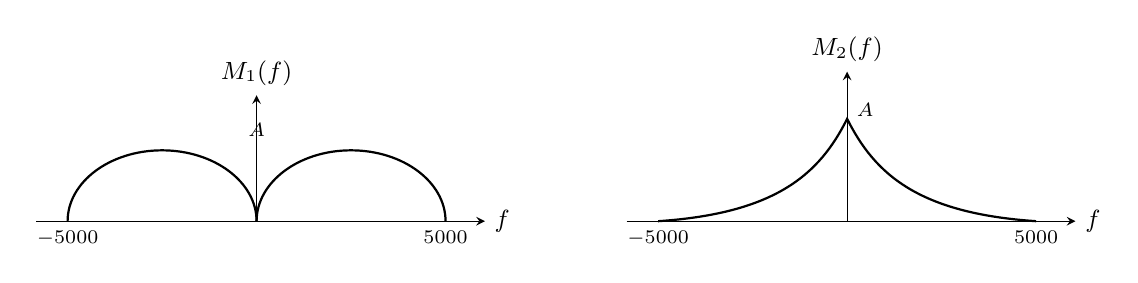
\begin{tikzpicture}[>=stealth,font=\small]
\draw[->] (-2.8,0) -- (2.9,0) node[right] {$f$};
\draw[->] (0,0) -- (0,1.6) node[above] {$M_1(f)$};
\draw[thick] (-2.4,0) arc[start angle=180,end angle=0,x radius=1.2,y radius=0.9];
\draw[thick] (0,0) arc[start angle=180,end angle=0,x radius=1.2,y radius=0.9];
\node[above] at (0,0.95) {\scriptsize $A$};
\node[below] at (-2.4,0) {\scriptsize $-5000$};
\node[below] at (2.4,0) {\scriptsize $5000$};
\begin{scope}[xshift=7.5cm]
\draw[->] (-2.8,0) -- (2.9,0) node[right] {$f$};
\draw[->] (0,0) -- (0,1.9) node[above] {$M_2(f)$};
\draw[thick] (-2.4,0) .. controls (-0.9,0.1) and (-0.35,0.6) .. (0,1.3) .. controls (0.35,0.6) and (0.9,0.1) .. (2.4,0);
\node[above right] at (0,1.2) {\scriptsize $A$};
\node[below] at (-2.4,0) {\scriptsize $-5000$};
\node[below] at (2.4,0) {\scriptsize $5000$};
\end{scope}
\end{tikzpicture}
\end{center}

\begin{center}
\begin{tikzpicture}[>=stealth,font=\small]
\node at (7.6,1.7) {Multiplexing};
\node[draw,circle,inner sep=1.5pt] (S) at (3.0,0) {$\Sigma$};
\draw[->] (0,1.6) -- (3.0,1.6) -- (S.north);
\node[below] at (0.5,1.6) {$m_1(t)$};
\node[draw,circle,inner sep=1pt] (X1) at (0.9,-1.3) {$\times$};
\draw[->] (-1.2,-1.3) -- (X1.west);
\node[below] at (0.9,-1.7) {$2\cos(20000\pi t)$};
\draw (X1.east) -- node[above] {\scriptsize $a$} (3.0,-1.3);
\draw[->] (3.0,-1.3) -- (S.south);
\node[turuncukalem,right] at (3.0,-0.95) {\scriptsize $x_a(t)$};
\node[draw,circle,inner sep=1pt] (X2) at (6.0,0) {$\times$};
\draw[->] (S.east) -- node[below] {\scriptsize $b$} (X2.west);
\node[turuncukalem,above] at (4.5,0.05) {\scriptsize $x_b(t)$};
\node[below] at (6.0,-0.6) {$2\cos(40000\pi t)$};
\draw[->] (X2.east) -- (8.6,0);
\node[below] at (7.8,0) {\scriptsize $c$};
\node[turuncukalem,above] at (7.8,0.05) {\scriptsize $x_c(t)$};
\end{tikzpicture}
\end{center}

\begin{gather*}
x_a(t)=2m_2(t)\cos(2\pi\,10\mathrm{k}\,t)\\
X_a(f)=M_2(f-10\mathrm{k})+M_2(f+10\mathrm{k})
\end{gather*}

\begin{center}
\begin{tikzpicture}[>=stealth,font=\small]
\draw[<->] (-5.2,0) -- (5.4,0);
\node[right] at (5.4,0) {$f$ (kHz)};
\draw[->] (0,0) -- (0,2);
\draw[thick] (-4.5,0) .. controls (-3.6,0.05) and (-3.2,0.5) .. (-3,1.2) .. controls (-2.8,0.5) and (-2.4,0.05) .. (-1.5,0);
\draw[thick] (1.5,0) .. controls (2.4,0.05) and (2.8,0.5) .. (3,1.2) .. controls (3.2,0.5) and (3.6,0.05) .. (4.5,0);
\draw[dashed] (0,1.2) -- (3.5,1.2);
\node[below] at (-4.5,0) {\scriptsize $-15$};
\node[below] at (-3,0) {\scriptsize $-10$};
\node[below] at (-1.5,0) {\scriptsize $-5$};
\node[below] at (1.5,0) {\scriptsize $5$};
\node[below] at (3,0) {\scriptsize $10$};
\node[below] at (4.5,0) {\scriptsize $15$};
\end{tikzpicture}
\end{center}

\sayfa{8}
\begin{gather*}
x_b(t)=m_1(t)+x_a(t)=m_1(t)+2m_2(t)\cos(2\pi\,10\mathrm{k}\,t)\\
X_b(f)=M_1(f)+M_2(f-10\mathrm{k})+M_2(f+10\mathrm{k})
\end{gather*}

\begin{center}
\begin{tikzpicture}[>=stealth,font=\small]
\draw[->] (-3,0) -- (8,0) node[right] {$f$ (kHz)};
\draw[->] (0,0) -- (0,2.2) node[above] {$|X_b(f)|$};
\draw[thick] (0,0) arc[start angle=180,end angle=0,x radius=1.125,y radius=1.2];
\draw[thick] (2.25,0) .. controls (3.6,0.1) and (4.2,0.6) .. (4.5,1.2) .. controls (4.8,0.6) and (5.4,0.1) .. (6.75,0);
\draw[dashed] (-3,1.2) -- (7.4,1.2);
\node[below] at (2.25,0) {\scriptsize $5$};
\node[below] at (4.5,0) {\scriptsize $10$};
\node[below] at (6.75,0) {\scriptsize $15$};
\node[anchor=west] at (1.1,1.75) {\scriptsize simetriği};
\draw[->] (1.05,1.75) -- (0.08,1.75);
\end{tikzpicture}
\end{center}

\begin{gather*}
x_c(t)=2x_b(t)\cos(2\pi\,20\mathrm{k}\,t)\\
X_c(f)=X_b(f-20\mathrm{k})+X_b(f+20\mathrm{k})
\end{gather*}

\begin{center}
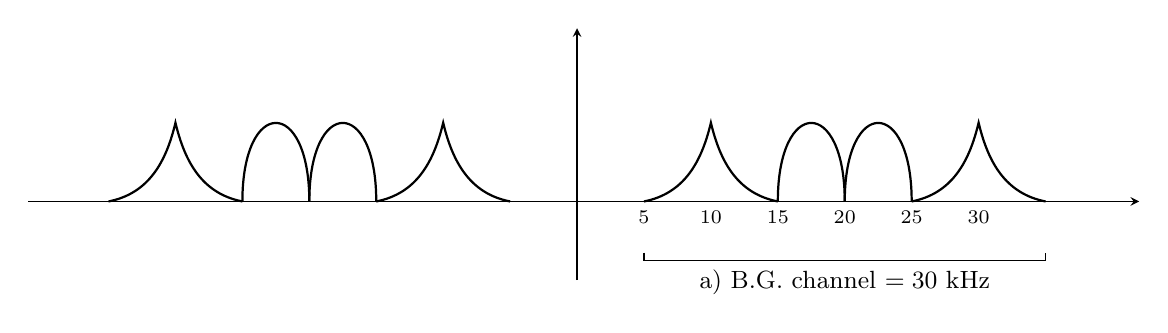
\begin{tikzpicture}[x=0.17cm,y=1cm,>=stealth,font=\small]
\draw[->] (-41,0) -- (42,0);
\draw[->] (0,-1) -- (0,2.2);
\begin{scope}
\draw[thick] (5,0) .. controls (8,0.1) and (9.3,0.5) .. (10,1) .. controls (10.7,0.5) and (12,0.1) .. (15,0);
\draw[thick] (15,0) .. controls (15,1.33) and (20,1.33) .. (20,0);
\draw[thick] (20,0) .. controls (20,1.33) and (25,1.33) .. (25,0);
\draw[thick] (25,0) .. controls (28,0.1) and (29.3,0.5) .. (30,1) .. controls (30.7,0.5) and (32,0.1) .. (35,0);
\end{scope}
\begin{scope}[xscale=-1]
\draw[thick] (5,0) .. controls (8,0.1) and (9.3,0.5) .. (10,1) .. controls (10.7,0.5) and (12,0.1) .. (15,0);
\draw[thick] (15,0) .. controls (15,1.33) and (20,1.33) .. (20,0);
\draw[thick] (20,0) .. controls (20,1.33) and (25,1.33) .. (25,0);
\draw[thick] (25,0) .. controls (28,0.1) and (29.3,0.5) .. (30,1) .. controls (30.7,0.5) and (32,0.1) .. (35,0);
\end{scope}
\node[below] at (5,0) {\scriptsize $5$};
\node[below] at (10,0) {\scriptsize $10$};
\node[below] at (15,0) {\scriptsize $15$};
\node[below] at (20,0) {\scriptsize $20$};
\node[below] at (25,0) {\scriptsize $25$};
\node[below] at (30,0) {\scriptsize $30$};
\draw (5,-0.65) -- (5,-0.75) -- (35,-0.75) -- (35,-0.65);
\node[below] at (20,-0.75) {a) B.G. channel $=30$ kHz};
\end{tikzpicture}
\end{center}

\begin{center}
\begin{tikzpicture}[>=stealth,font=\small]
\node[turuncukalem] at (1.9,1.35) {\scriptsize demodülasyon};
\node[anchor=east] at (0,0) {$x_c(t)$};
\node[draw,circle,inner sep=1pt] (X3) at (1.6,0) {$\times$};
\draw[->] (0.05,0) -- (X3.west);
\draw[->] (1.6,-1.0) -- (X3.south);
\node[below] at (1.6,-1.0) {\scriptsize $\cos(2\pi\,20\mathrm{kHz})$};
\draw (X3.east) -- node[above] {\scriptsize $d$} (3.6,0);
\node[draw,align=center,minimum width=2.0cm,minimum height=0.8cm] (A1) at (7.0,1.0) {AGF\\ B.G.: 5kHz};
\draw[->] (3.6,0) -- (3.6,1.0) -- (A1.west);
\draw[->] (A1.east) -- (9.3,1.0) node[right] {$\hat m_1(t)$};
\node[draw,circle,inner sep=1pt] (X4) at (6.0,-1.6) {$\times$};
\draw (3.6,0) -- (3.6,-1.6);
\draw[->] (3.6,-1.6) -- node[above] {\scriptsize $e$} (X4.west);
\draw[->] (6.0,-2.3) -- (X4.south);
\node[below] at (6.0,-2.3) {\scriptsize $\cos(2\pi\,10\mathrm{k}\,t)$};
\node[draw,align=center,minimum width=2.0cm,minimum height=0.8cm] (A2) at (8.6,-1.6) {AGF\\ B.G.: 5kHz};
\draw[->] (X4.east) -- (A2.west);
\draw[->] (A2.east) -- (10.8,-1.6) node[right] {$\hat m_2(t)$};
\end{tikzpicture}
\end{center}

\begin{gather*}
x_d(t)=x_c(t)\cos(2\pi\,20\mathrm{k}\,t)\\
X_d(f)=\frac12 X_c(f-20\mathrm{k})+\frac12 X_c(f+20\mathrm{k})
\end{gather*}

\sekilnotu[8]{Sayfanın en altında $X_d(f)$ için spektrum taslağı (alt kenarda kesilmiş): eksen üzerinde solda, ortada ve sağda üç grup; her grup iki kubbe ve iki sivri tepeden oluşuyor. Ortadaki grubun iki kubbesi kırmızı kesikli köşeli parantezle çevrilmiş; kırmızı etiket: $X_d(f)\rightarrow\hat M_1(f)$ (oklu).}

\sayfa{9}
\begin{gather*}
x_e(t)=x_d(t)\cos(2\pi\,10\mathrm{k}\,t)\\
\longrightarrow\ X_e(f)=\frac12 X_d(f-10\mathrm{k})+\frac12 X_d(f+10\mathrm{k})
\end{gather*}

\begin{center}
\begin{tikzpicture}[>=stealth,font=\small]
\draw[->] (-4,0) -- (4.2,0);
\draw[->] (0,-0.5) -- (0,1.7);
\draw[thick] (-1,0) .. controls (-0.5,0.05) and (-0.2,0.5) .. (0,1.2) .. controls (0.2,0.5) and (0.5,0.05) .. (1,0);
\draw[dashed,kirmizikalem] (-1.1,0) -- (-1.1,1.3) -- (-0.8,1.3);
\draw[dashed,kirmizikalem] (1.1,0) -- (1.1,1.3) -- (0.8,1.3);
\node[kirmizikalem,anchor=west] at (1.25,1.45) {\scriptsize $\hat M_2(f)$};
\end{tikzpicture}
\end{center}

\end{document}
